% $Id: conclusion.tex 
% !TEX root = main.tex

%%
\section{Adaptive \ac{RL} Agents with Changing Behavior}
\label{sec:implementation}

This section introduces \adaptiverl, our proposed approach for enabling \ac{RL} agents to dynamically adapt their behavior in response to evolving environmental conditions. Our method allows agents to pursue varying objectives throughout their operational lifespan and acquire new capabilities as tasks change over time. The implementation is publicly available\footnote{Available at: \url{https://github.com/rulas99/rl_uniandes}}.

The conceptual foundation of \adaptiverl aligns with the ideas proposed by~\citet{abel2023definitioncontinualreinforcementlearning}, emphasizing continual adaptation rather than convergence to a fixed solution. We extend tabular Q-learning by integrating adaptive mechanisms that enable agents to dynamically adjust their learning strategies in response to detected environmental changes. Similar to the approach described by~\citet{norman2024firstexploreexploitmetalearningsolve}, our agent thoroughly explores the environment each time a change is detected, subsequently exploiting the acquired knowledge. This strategy facilitates rapid convergence to new environment configurations without entirely discarding previously learned knowledge.

To enable dynamic behavioral adaptation, we introduce adaptive mechanisms that adjust the agent’s learning rate and exploration rate in conjunction with a concept drift detection strategy. By continuously monitoring and responding to changes in the environment, our agent can autonomously modify its learning process at runtime to maintain effective goal pursuit. This capability positions our approach within the class of self-adaptive systems (SAS), as defined by~\citet{sasreview}, ensuring continual adaptation and resilience in non-stationary contexts.

We dynamically adjust the learning rate based on the Temporal Difference (TD) error, as defined in~\eqref{eq:td_error}.

\begin{equation}
    \label{eq:td_error}
    TD_{error} = r_{t+1} + \gamma \cdot \underset{a}{\max} Q(s_{t+1}, a) - Q(s_t, a_t)
\end{equation}

This error quantifies the difference between the agent’s predicted reward and the actual reward received. The dynamic learning rate ($\alpha^*$) is then adjusted based on the TD error, as defined in~\eqref{eq:dynamic_learning_rate}.

\begin{equation}
    \label{eq:dynamic_learning_rate}
    \alpha^* = \alpha + (\alpha_{\max}-\alpha) \cdot \frac{1}{1 + e^{-(|TD_{error}|-k)}}
\end{equation}

In this formulation, $\alpha$ denotes the base learning rate (e.g., 0.1), while $\alpha_{\max}$ specifies its upper bound (e.g., 0.99). The parameter $k$ controls the sensitivity of the learning rate to the TD error, with higher values resulting in reduced sensitivity; thus, $k$ must be carefully tuned according to the specific characteristics of the environment and learning context. High TD errors induce a larger learning rate, enabling faster updates during exploration, whereas lower TD errors yield a more stable and conservative learning process during exploitation phases. In Figure~\ref{fig:alpha}, we illustrate the behavior of the dynamic learning rate ($\alpha^*$) in our Non-Stationary GridWorld experiments.

\begin{figure*}
    \centering
    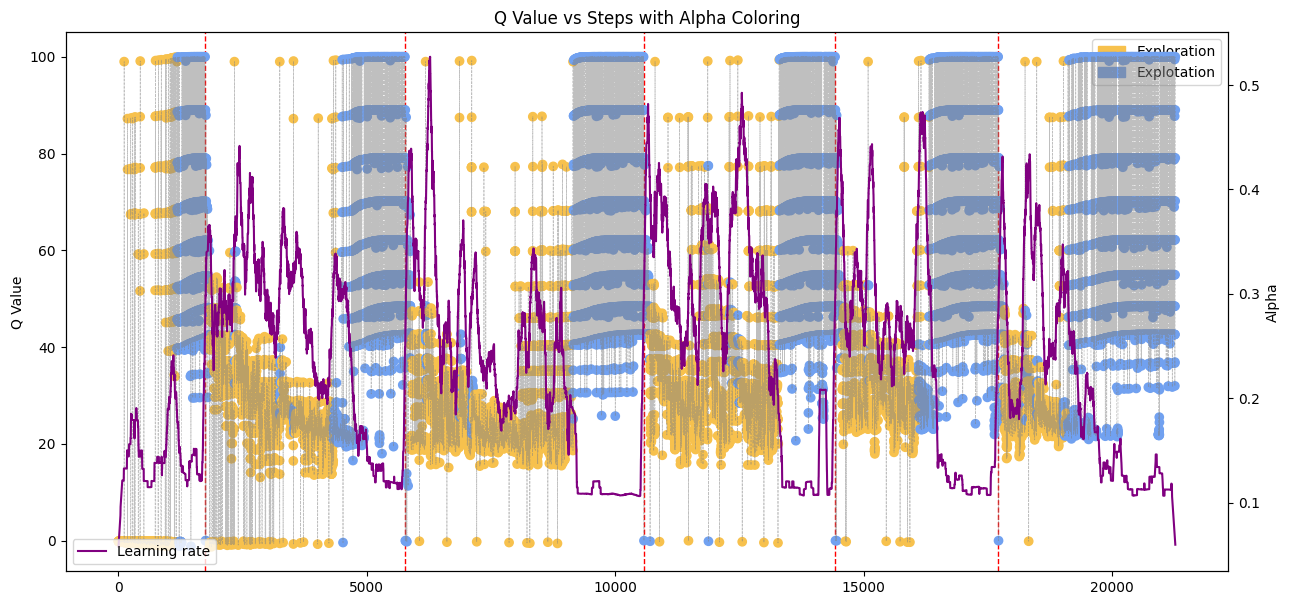
\includegraphics[width=\textwidth]{figures/alpha.png}
    \caption{Behavior of dynamic learning rate ($\alpha^*$) over Non-Stationary GridWorld experiments. Notice how $\alpha^*$ increases when the agent is exploring $\rightarrow$ high TD error and decreases when the agent is exploiting (low TD error), achieving a fast convergence during exploration and a stable learning during exploitation.}
    \label{fig:alpha}
\end{figure*}

Following the methodologies of~\citet{mignon2017adaptive} and~\citet{networkdynamicrl}, we implement the PH-test to detect significant shifts in the reward distribution at the end of each episode. The PH-test calculates a cumulative difference between observed rewards and the running mean reward, incorporating a sensitivity parameter ($\delta$). A concept drift (environmental change) is flagged when this cumulative difference surpasses a predefined threshold. Selecting an appropriate threshold value is crucial, as it determines the sensitivity of drift detection. Higher thresholds result in more conservative detection, while lower thresholds increase sensitivity to changes, this value must be selected based on the magnitude order of rewards and posible changes over them.

Building on the concept drift detection mechanism and inspired by~\citet{mignon2017adaptive}, we adaptively increase the exploration rate ($\varepsilon$) whenever the PH-test detects a concept drift. This approach promotes exploration immediately following environmental changes, enabling the agent to acquire new knowledge by temporarily adopting an exploration-focused policy. To ensure adequate exploration, the agent maintains this elevated exploration rate for a period (until rewards stabilize, i.e., no further drifts are detected) before $\varepsilon$ resumes its usual decay toward a minimal value, thereby returning to the exploitation phase.

This adaptive exploration mechanism ensures the agent maintains an effective balance between exploring new environment dynamics and leveraging previously acquired knowledge. It is crucial to sustain high exploration levels after consistent concept drift detection, so the agent can learn new policies without forgetting previously learned ones. In Figure~\ref{fig:dynamic-eps}, we illustrate the behavior of the dynamic exploration rate ($\varepsilon^*$) in our Non-Stationary GridWorld experiments

\begin{figure*}
    \centering
    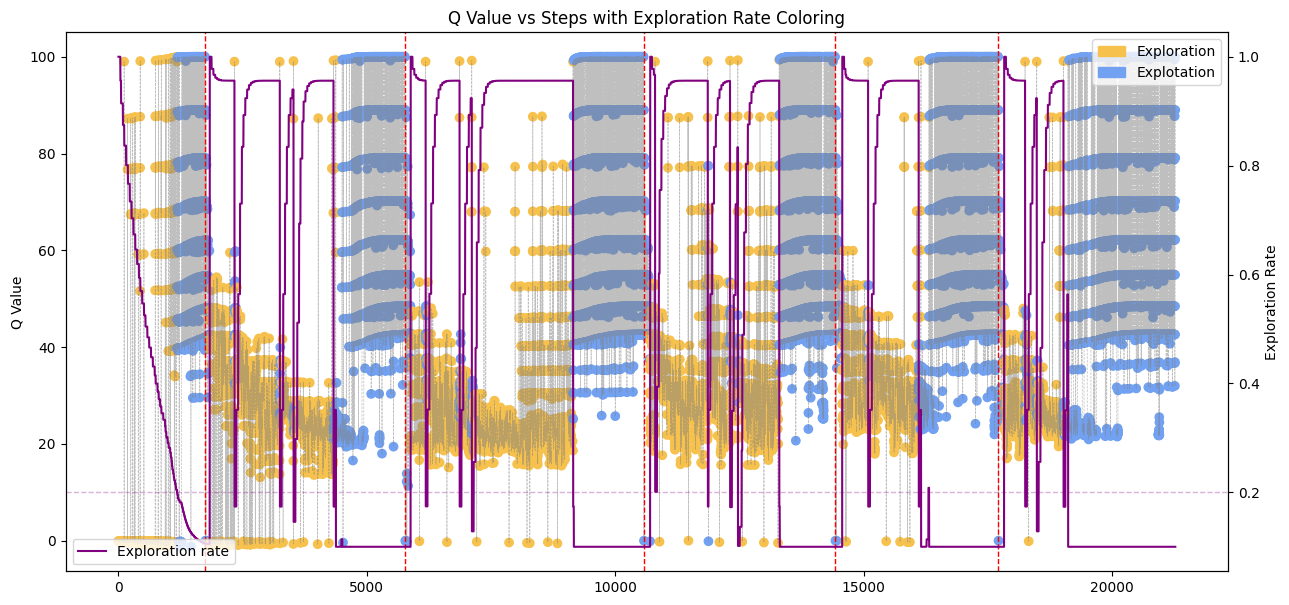
\includegraphics[width=\textwidth]{figures/epsilon.png}
    \caption{Behavior of the dynamic exploration rate ($\varepsilon^*$) in Non-Stationary GridWorld experiments. Notice how $\varepsilon^*$ increases each time a concept drift is detected by the PH-test and remains high until the agent consistently achieves the expected rewards (i.e., no further concept drift and stable rewards). Afterward, $\varepsilon^*$ begins to decay toward its minimum value allowing to explode the acquired knowledge.}
    \label{fig:dynamic-eps}
\end{figure*}

These adaptive mechanisms equip the agent to effectively manage learning under varying and unpredictable conditions, enabling continuous adaptation and efficient knowledge transfer between different environmental states. This approach allows the agent to rapidly respond to new information without discarding previously learned knowledge, achieving greater resilience and performance stability over its lifespan. In continous, we present a GridWorld example to illustrate \adaptiverl's behavior in am environment with non-stationary reward function and compare it with a standard Q-learning agent.

%%%%
\subsection{Agent Adaptation to Different Goals}
\label{sec:experiments}

To evaluate \adaptiverl's ability to adapt to environmental changes involving a non-stationary reward function—and to compare its performance with traditional Q-learning—we design a $9\times 9$ GridWorld environment. In this setting, each cell yields a reward of $-1$, except for the goal state. The agent, starting at the center of the grid, can move in four directions (up, down, left, right) and receives a positive reward of $+100$ only upon reaching the goal cell, which is initially located at the top-left corner. Every 300 episodes, after the agent is expected to have learned the optimal policy, we introduce a concept drift by relocating the goal cell to the diagonally opposite corner (bottom right), alternating the goal position between the top-left and bottom-right corners. This process is repeated for a total of 1500 episodes, requiring the agent to detect and rapidly adapt its policy to achieve convergence following each drift event. Figure~\ref{fig:r-change} shows the GridWorld environment and the induced concept drift configuration for the experiment.

\begin{figure*}
    \centering
    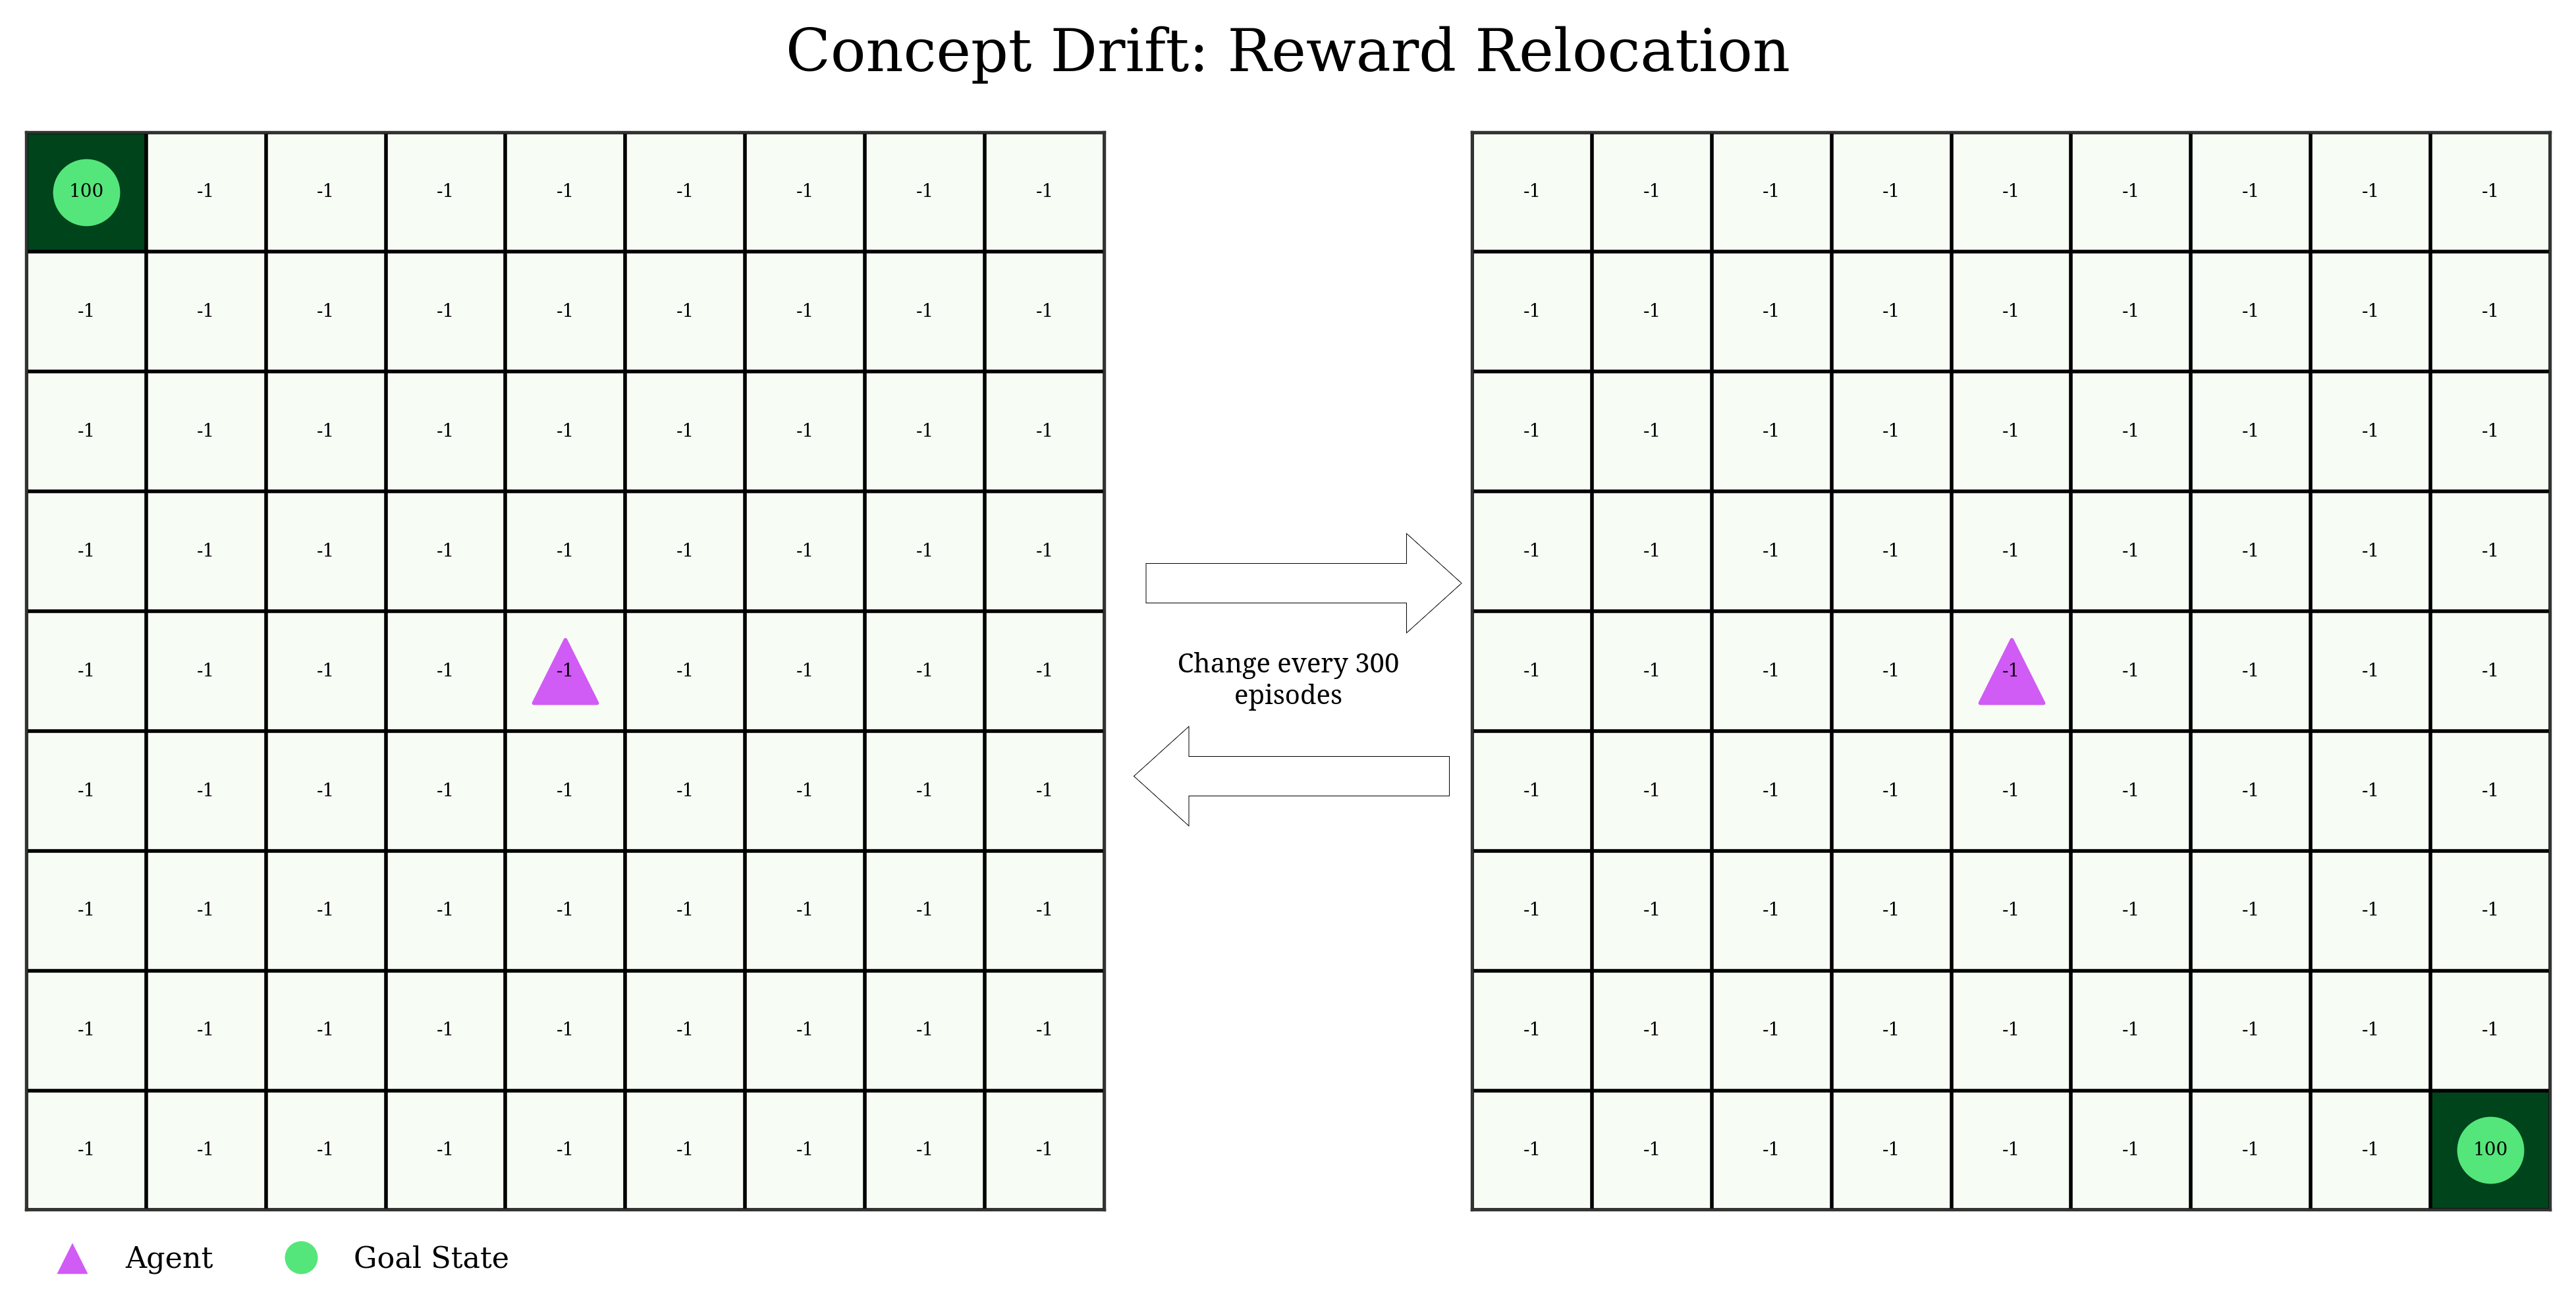
\includegraphics[width=\textwidth]{figures/r_change.png}
    \caption{GridWorld environment with non-stationary reward function. The agent starts at the center, and its goal is initially located at the top-left corner. Every 300 episodes, the goal is moved to its diagonal opposite, so the goal state alternates between the top-left and bottom-right corners. The agent is expected to detect the concept drift and rapidly adapt its policy to achieve convergence after each drift event.}
    \label{fig:r-change}
\end{figure*}

We run the experiment a thousand times with two agents: a standard Q-learning agent and an \adaptiverl agent. The standard Q-learning agent uses a fixed learning rate ($\alpha=0.1$) and a fixed exploration decayment rate ($\varepsilon=0.1$), while the \adaptiverl agent employs the adaptive mechanisms described in Section~\ref{sec:implementation}. We evaluate the agents' performance based on the times it converged to a optimal policy for each reward change, how many steps it takes and the total steps to complete de 1500 episodes. The Table 1

\begin{table}
    \centering
    \caption{Table with multirow and multicolumns definitions}
    \resizebox{1.01\columnwidth}{!}{

\begin{tabular}{l | cccccc }
\toprule
\textbf{Algorithm} & \textbf{\acs{LOC}} & \textbf{Loops} & \textbf{Conditionals} & \textbf{Parameters} & \textbf{Data structures} & \textbf{\acs{CFG} nodes} \\
\toprule
\multicolumn{2}{l}{\textbf{Sorting algorithms}} \\
Bubble sort & 19 & 2 & 1 & array & \multirow{3}{*}{-} & 9 \\
Gnone sort & 16 & 1 & 1 & array &  & 8 \\
Merge sort  & 54 & 5 & 2 & array &  & 27\\
Quick sort  & 36 & 2 & 2 & array & stack & 13\\
\midrule
\multicolumn{2}{l}{\textbf{Search algorithms}} \\
Binary search & 16 & 1 & 2 & array & - & 9\\
Linear search & 10 & 1 & 1 & array & - & 8\\
\midrule
\multicolumn{2}{l}{\textbf{Aggregation algorithms}} \\
Min & 10 & 1 & 1 & array & - & 9\\
Max & 10 & 1 & 1 & array & - & 9\\
Sum & 7 & 1 & 0 & array & - & 4\\
Sum odd & 9 & 1 & 1 & array & - & 6\\
\bottomrule
\end{tabular}

}
    \label{tab:multi}
  \end{table}

\begin{figure*}
    \centering
    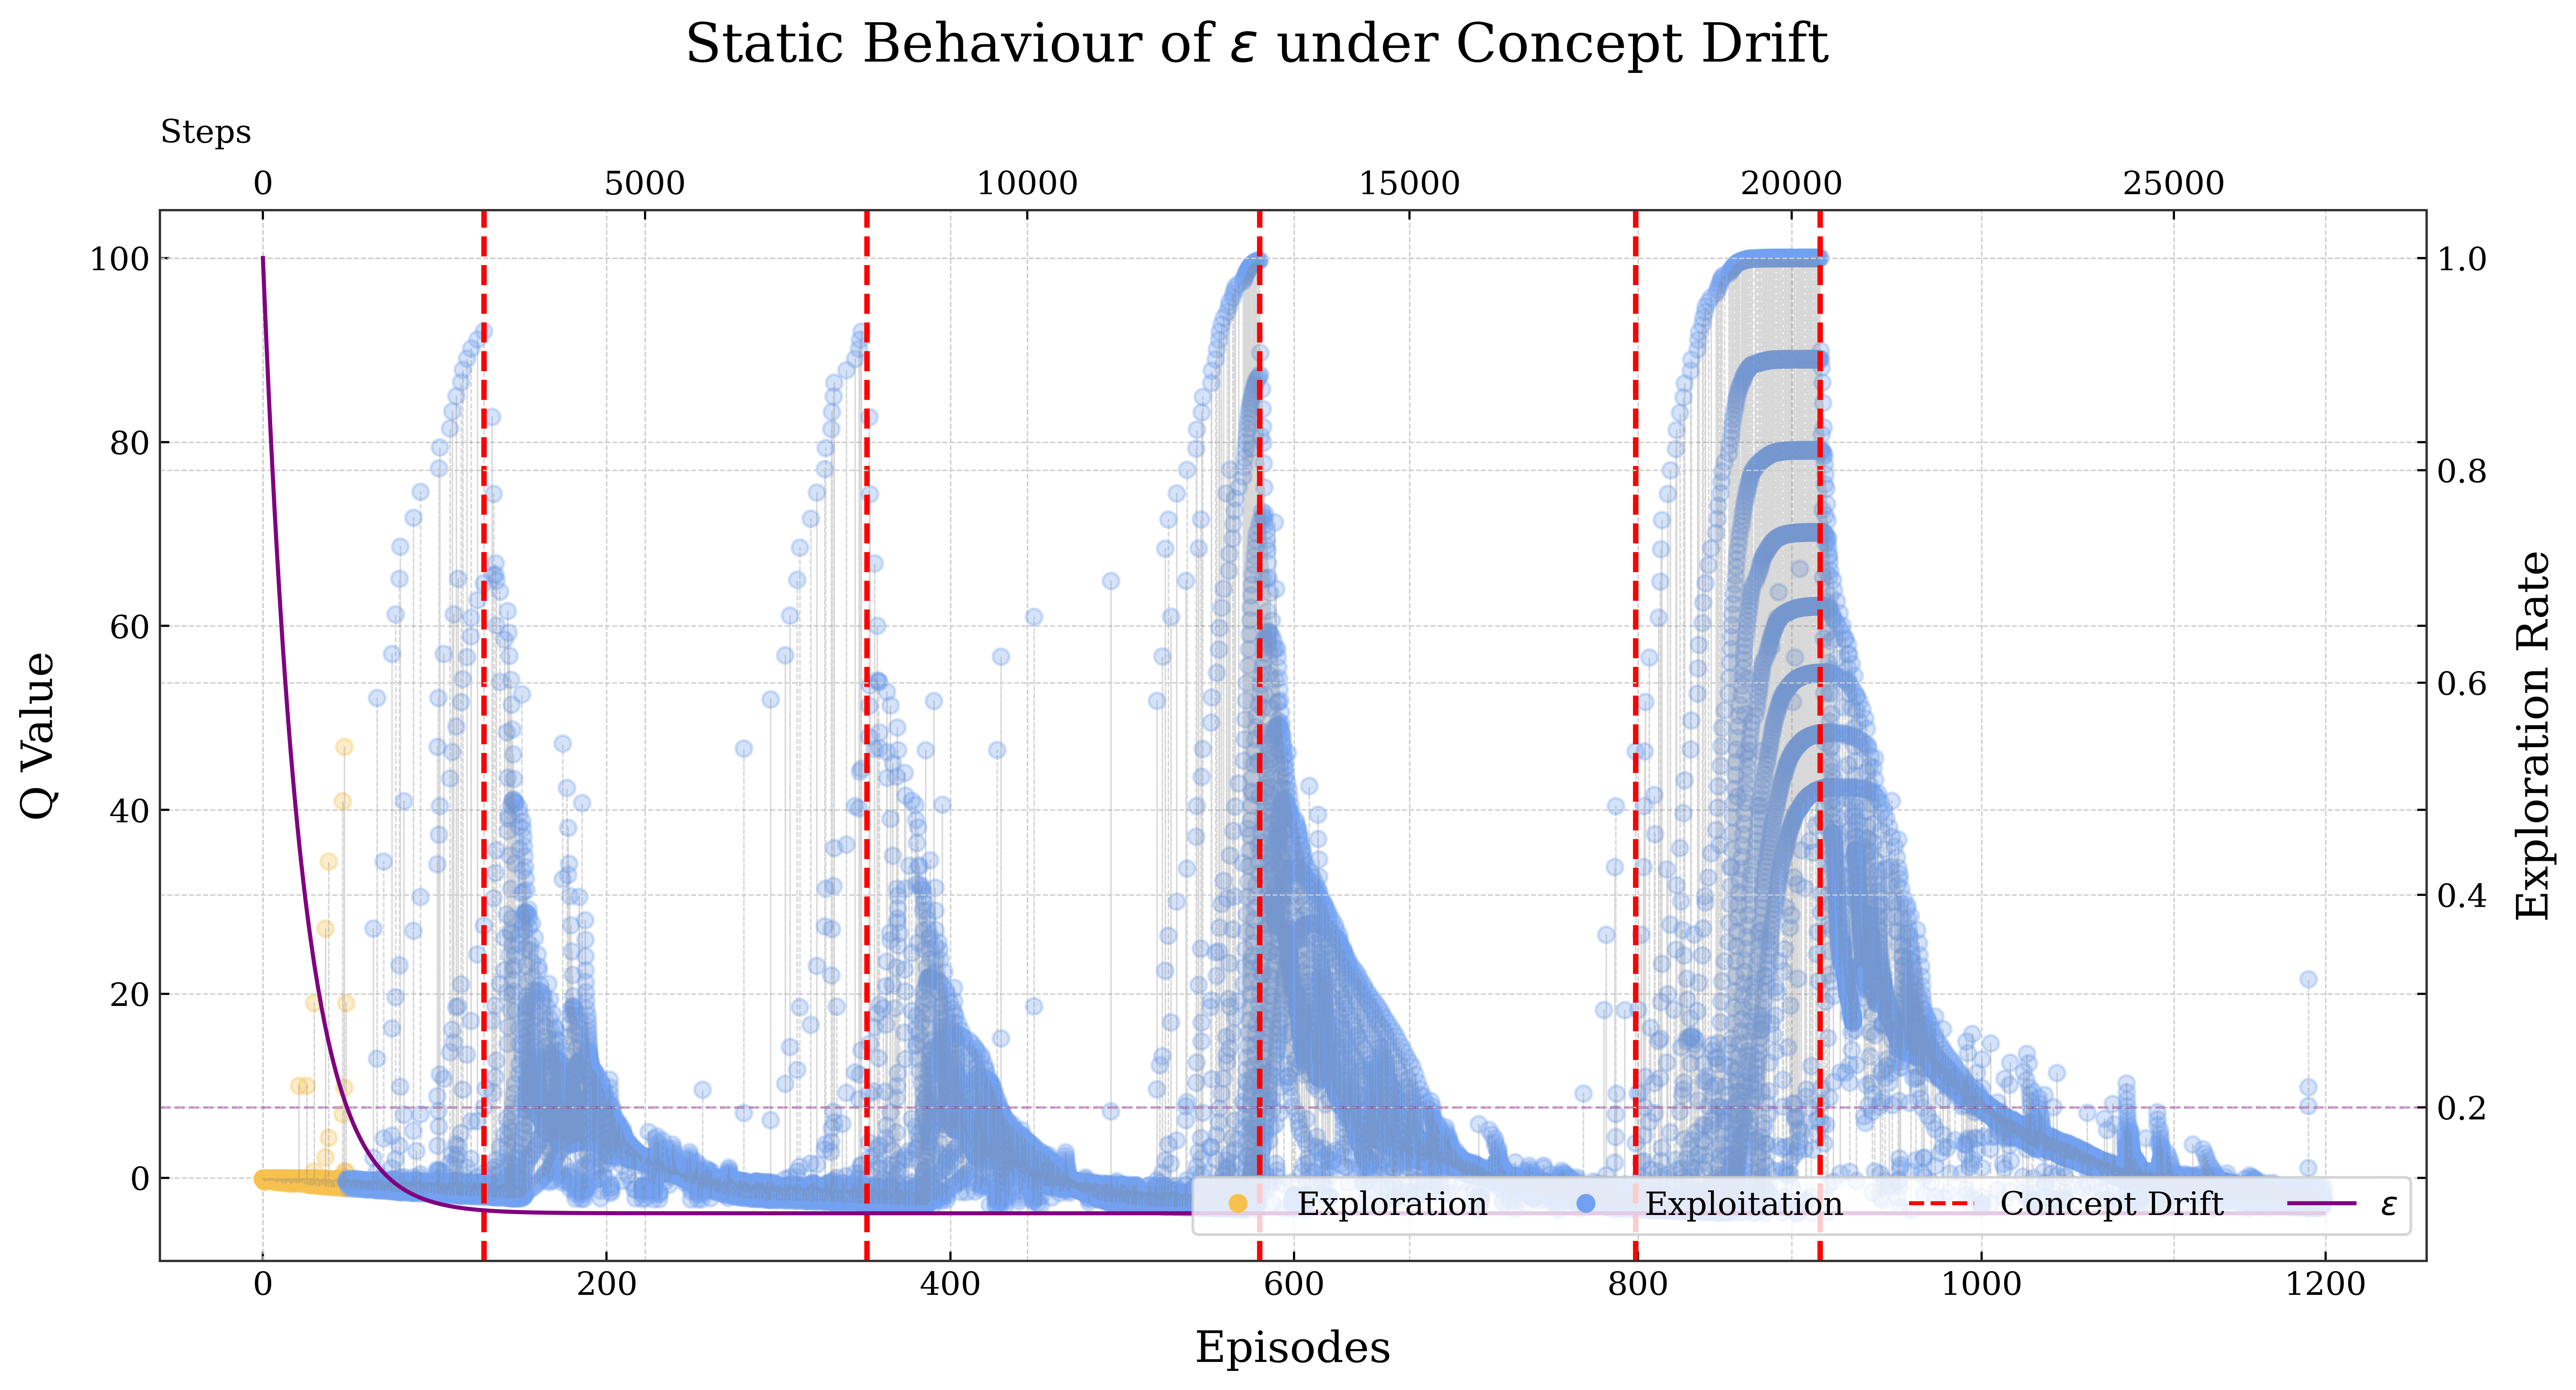
\includegraphics[width=\textwidth]{figures/trad_eps.png}
    \caption{Behavior of the dynamic exploration rate ($\varepsilon^*$) in Non-Stationary GridWorld experiments. Notice how $\varepsilon^*$ increases each time a concept drift is detected by the PH-test and remains high until the agent consistently achieves the expected rewards (i.e., no further concept drift and stable rewards). Afterward, $\varepsilon^*$ begins to decay toward its minimum value allowing to explode the acquired knowledge.}
    \label{fig:static-eps}
\end{figure*}

%%%%
\subsection{Agent acquisition of new capabilities}


\endinput

